\documentclass[12pt]{article}
\usepackage{lingmacros}
\usepackage{tree-dvips}
\usepackage{graphicx}
\usepackage{amsmath}
\usepackage{amssymb}
\usepackage{tikz}
\usepackage{color}

\begin{document}

\title{Performance Characterization of Evaluating Hessian Using Automatic Differentiation Algorithms}
\maketitle
\paragraph{Introduction}
\paragraph{Algorithms}
\paragraph{Testing philosphy}
\paragraph{Results}
\paragraph{Conclusion}

\appendix
\section{The old stuff}
\subsection{Randomized Hessians, Analyzing Program Structures}
\label{sec-perf-rand}

\label{sec-perf-random}

\paragraph{A) Test setting and objectives.}
The objectives of the tests discussed in this section are distinct from
the objectives of the tests presented in Sections~\ref{sec-perf-syn} and \ref{sec-perf-opt}.
Here we construct testcases specially designed to enable in-depth
empirical analysis of {\em programming} and {\em structural factors} that 
determine the performance of the  different Hessian algorithms. 
To construct the testcases, we wrote a simple code that works as follows. 
Let the number of rows in the target Hessian matrix be $n$, and
let the average number of nonzeros per row, $\bar{\rho}$, be fixed.
In a loop over the $n$ rows, for each row $i$, 
we pick $\frac{\bar{\rho}}{2}$ column indices at random to insert nonzero values into the Hessian.    
We do this by using a deterministic random number generator to identify a column index $j$ and {\em the basic operation} 
$\tt 1.0+x[i]*x[j]$ to create the nonzero entry in the location $H(i,j)$. 
Further, a statement in the loop consists of the sum of $k$ basic operations added to the dependent variable $y$. We also permit a statement to be repeated $s$ times in a loop. Thus the total number of basic operations per loop is the product of the number of statements per loop $s$ and the number of basic operations per statement $k$. Varying $s$ and $k$ gives us the flexibility to implement the same function in different ways.

Within this setting, we can control the number of rows in the Hessian matrix, the density/sparsity of the Hessian, and the complexity of the function evaluation. Because we build
the objective function in a ``separable'' fashion, in the complexity of 
\textsc{Livarh} given by Expression~\eqref{eq-ub1}, $d_i$ is constant, which means the complexity of \textsc{Livarh} is proportional to just $l$, the complexity of the function 
evaluation in this case.
(We include pseudocode for the random Hessian generator we described in the Appendix~\ref{sec-random-code}.)   


\paragraph{B) Dependence on number of basic operations per statement.}

As discussed in Section~\ref{sec-preacc-analysis}, the performance of \textsc{Livarhacc} depends on how complex a statement is. We would like to measure this dependence
and see if the other methods' performance also depends on the complexity of a statement. We fix the size of the Hessian as $n=20,000$, the average number of nonzeros per row as $\overline{\rho} = 6$, and the total number of basic operations per loop as $B=128$.
We vary the number of basic operations per statement ($k$) while keeping $B=k s$ fixed, where $s$ is the number of statements per loop. We use a fixed seed in the random number generator,
so we always get the same nonzero structure in the Hessian. 

\begin{figure}[htbp]
\centering
\begin{minipage}[b]{0.48\linewidth}
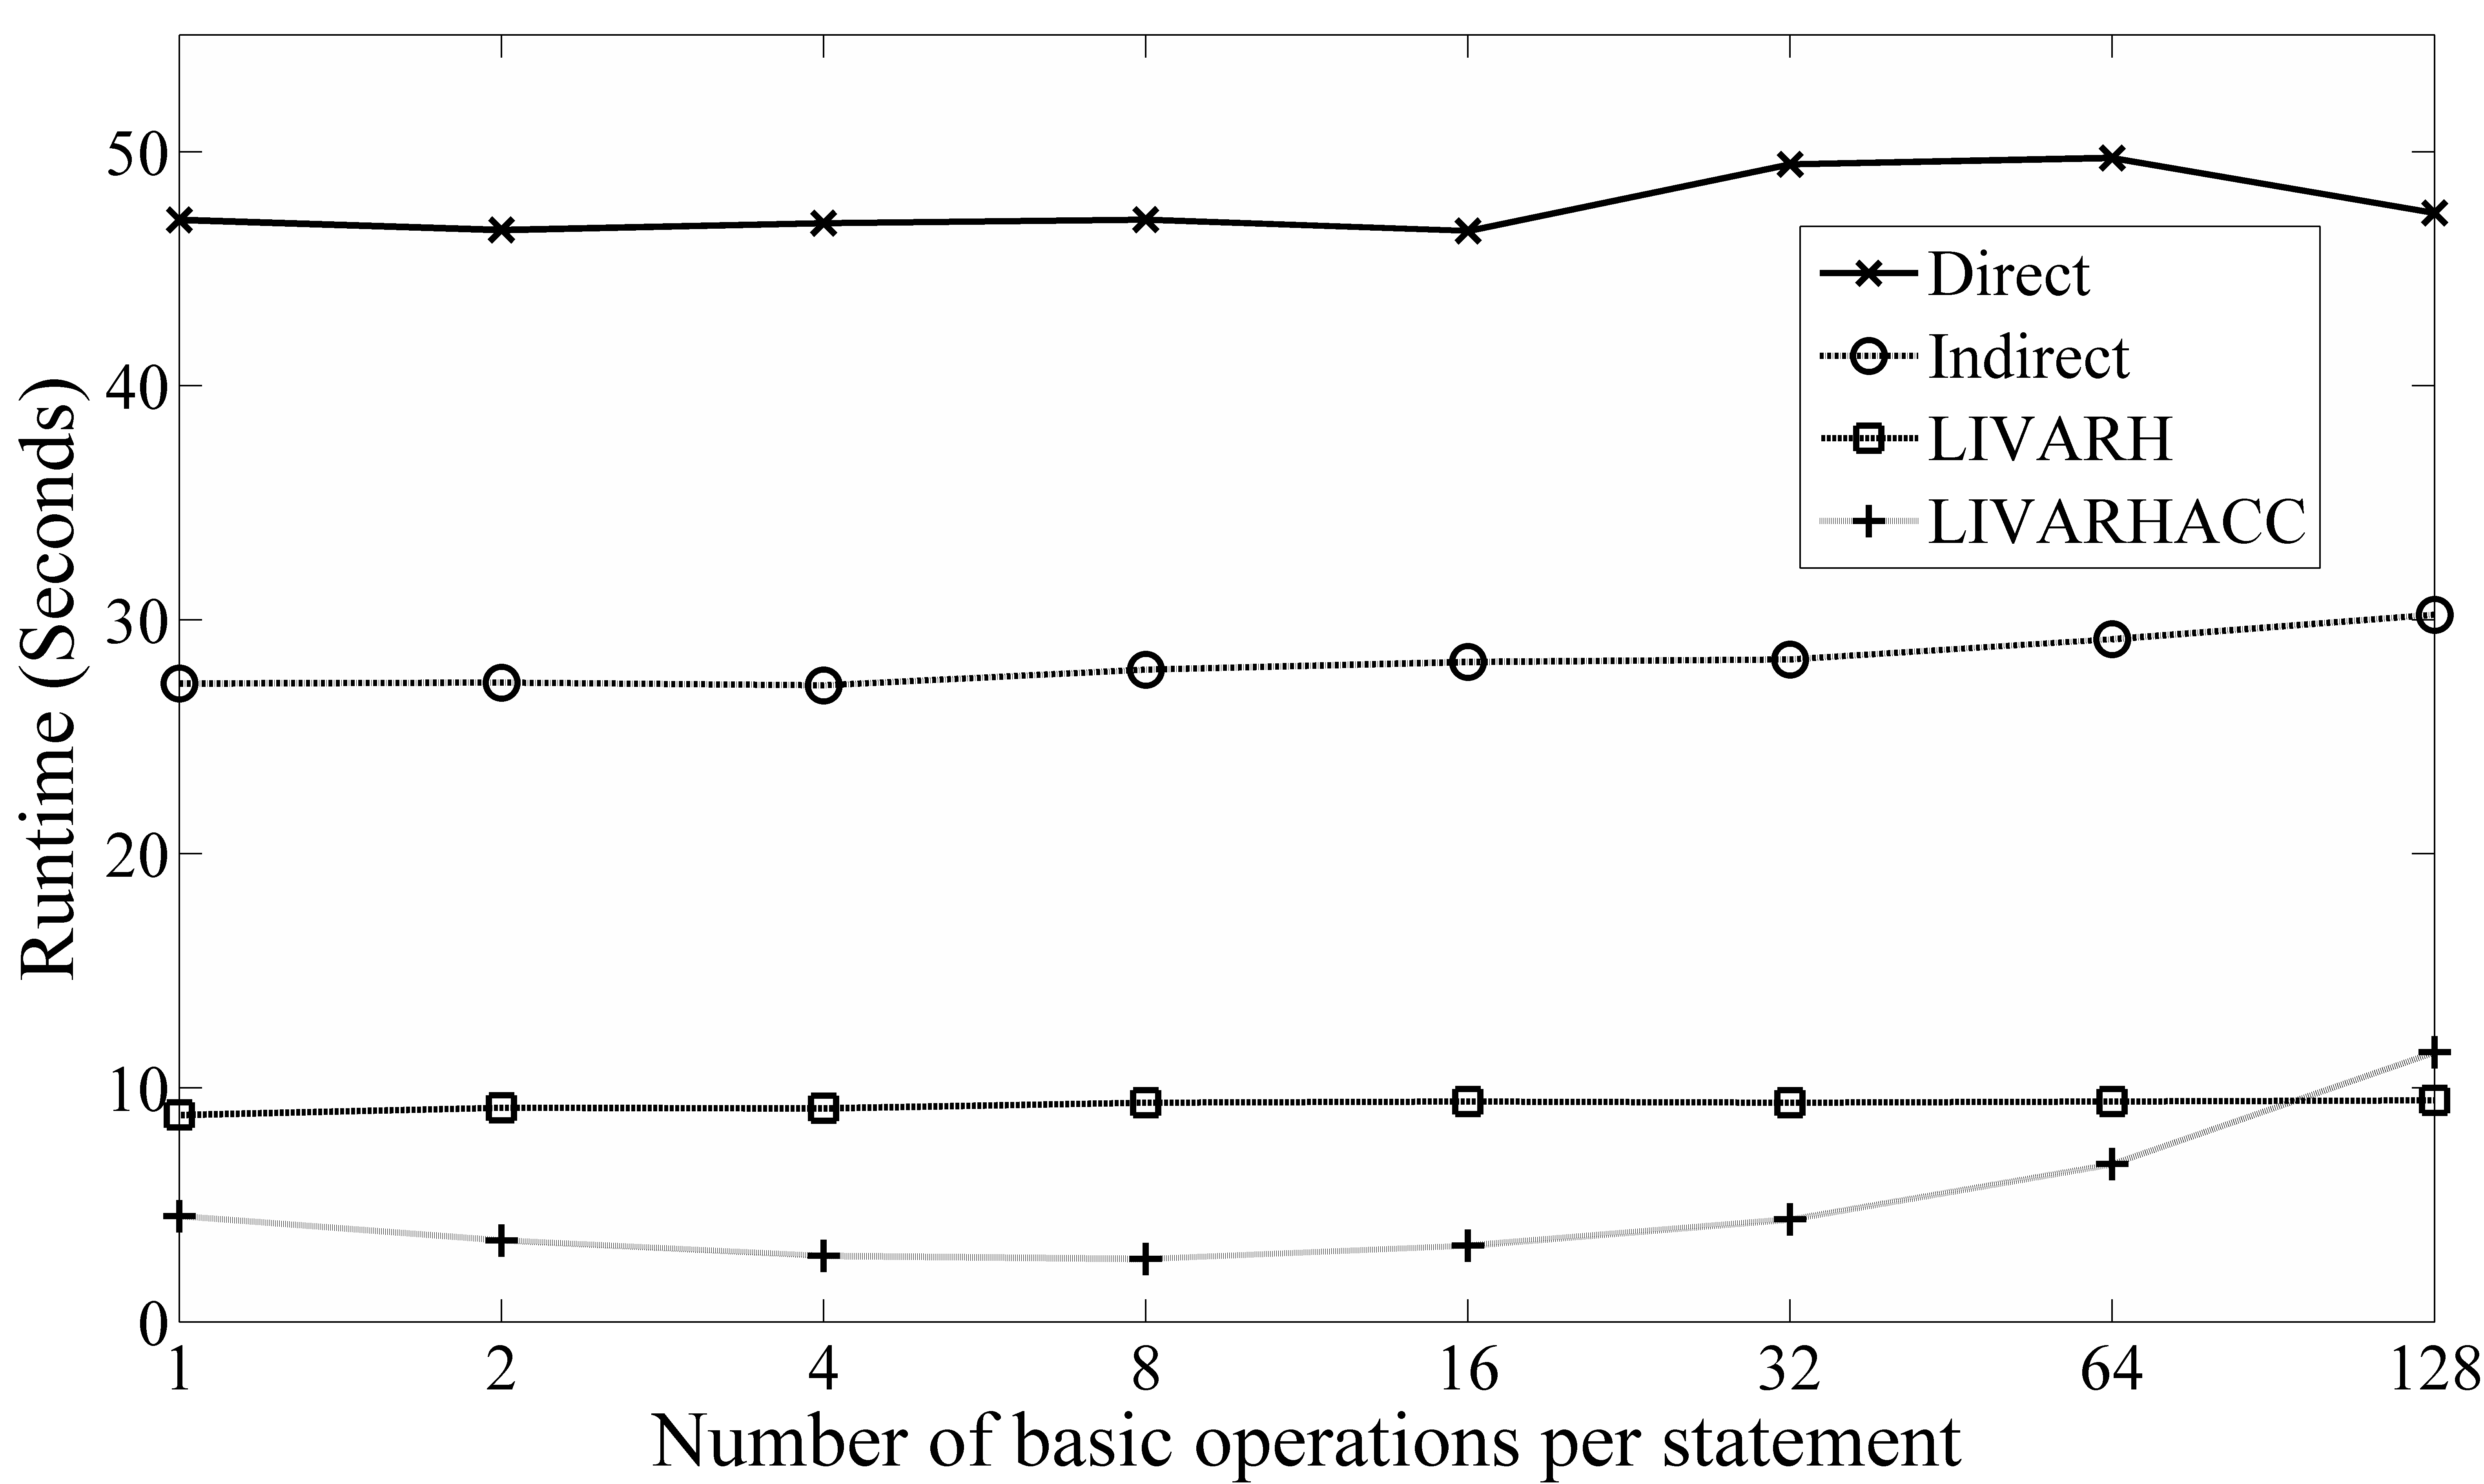
\includegraphics[width=1\textwidth]{figures/HRfig1BW}
\caption[ Runtime Variation under Different Number of Basic Operations per Loop]
{Runtime variation under different number of basic operations per loop.
Fixed parameters: $n=20,000$, $\overline{\rho} = 6$, $B=128$. }
\label{fig:random-fig1}
\end{minipage}
\quad
\begin{minipage}[b]{0.48\linewidth}
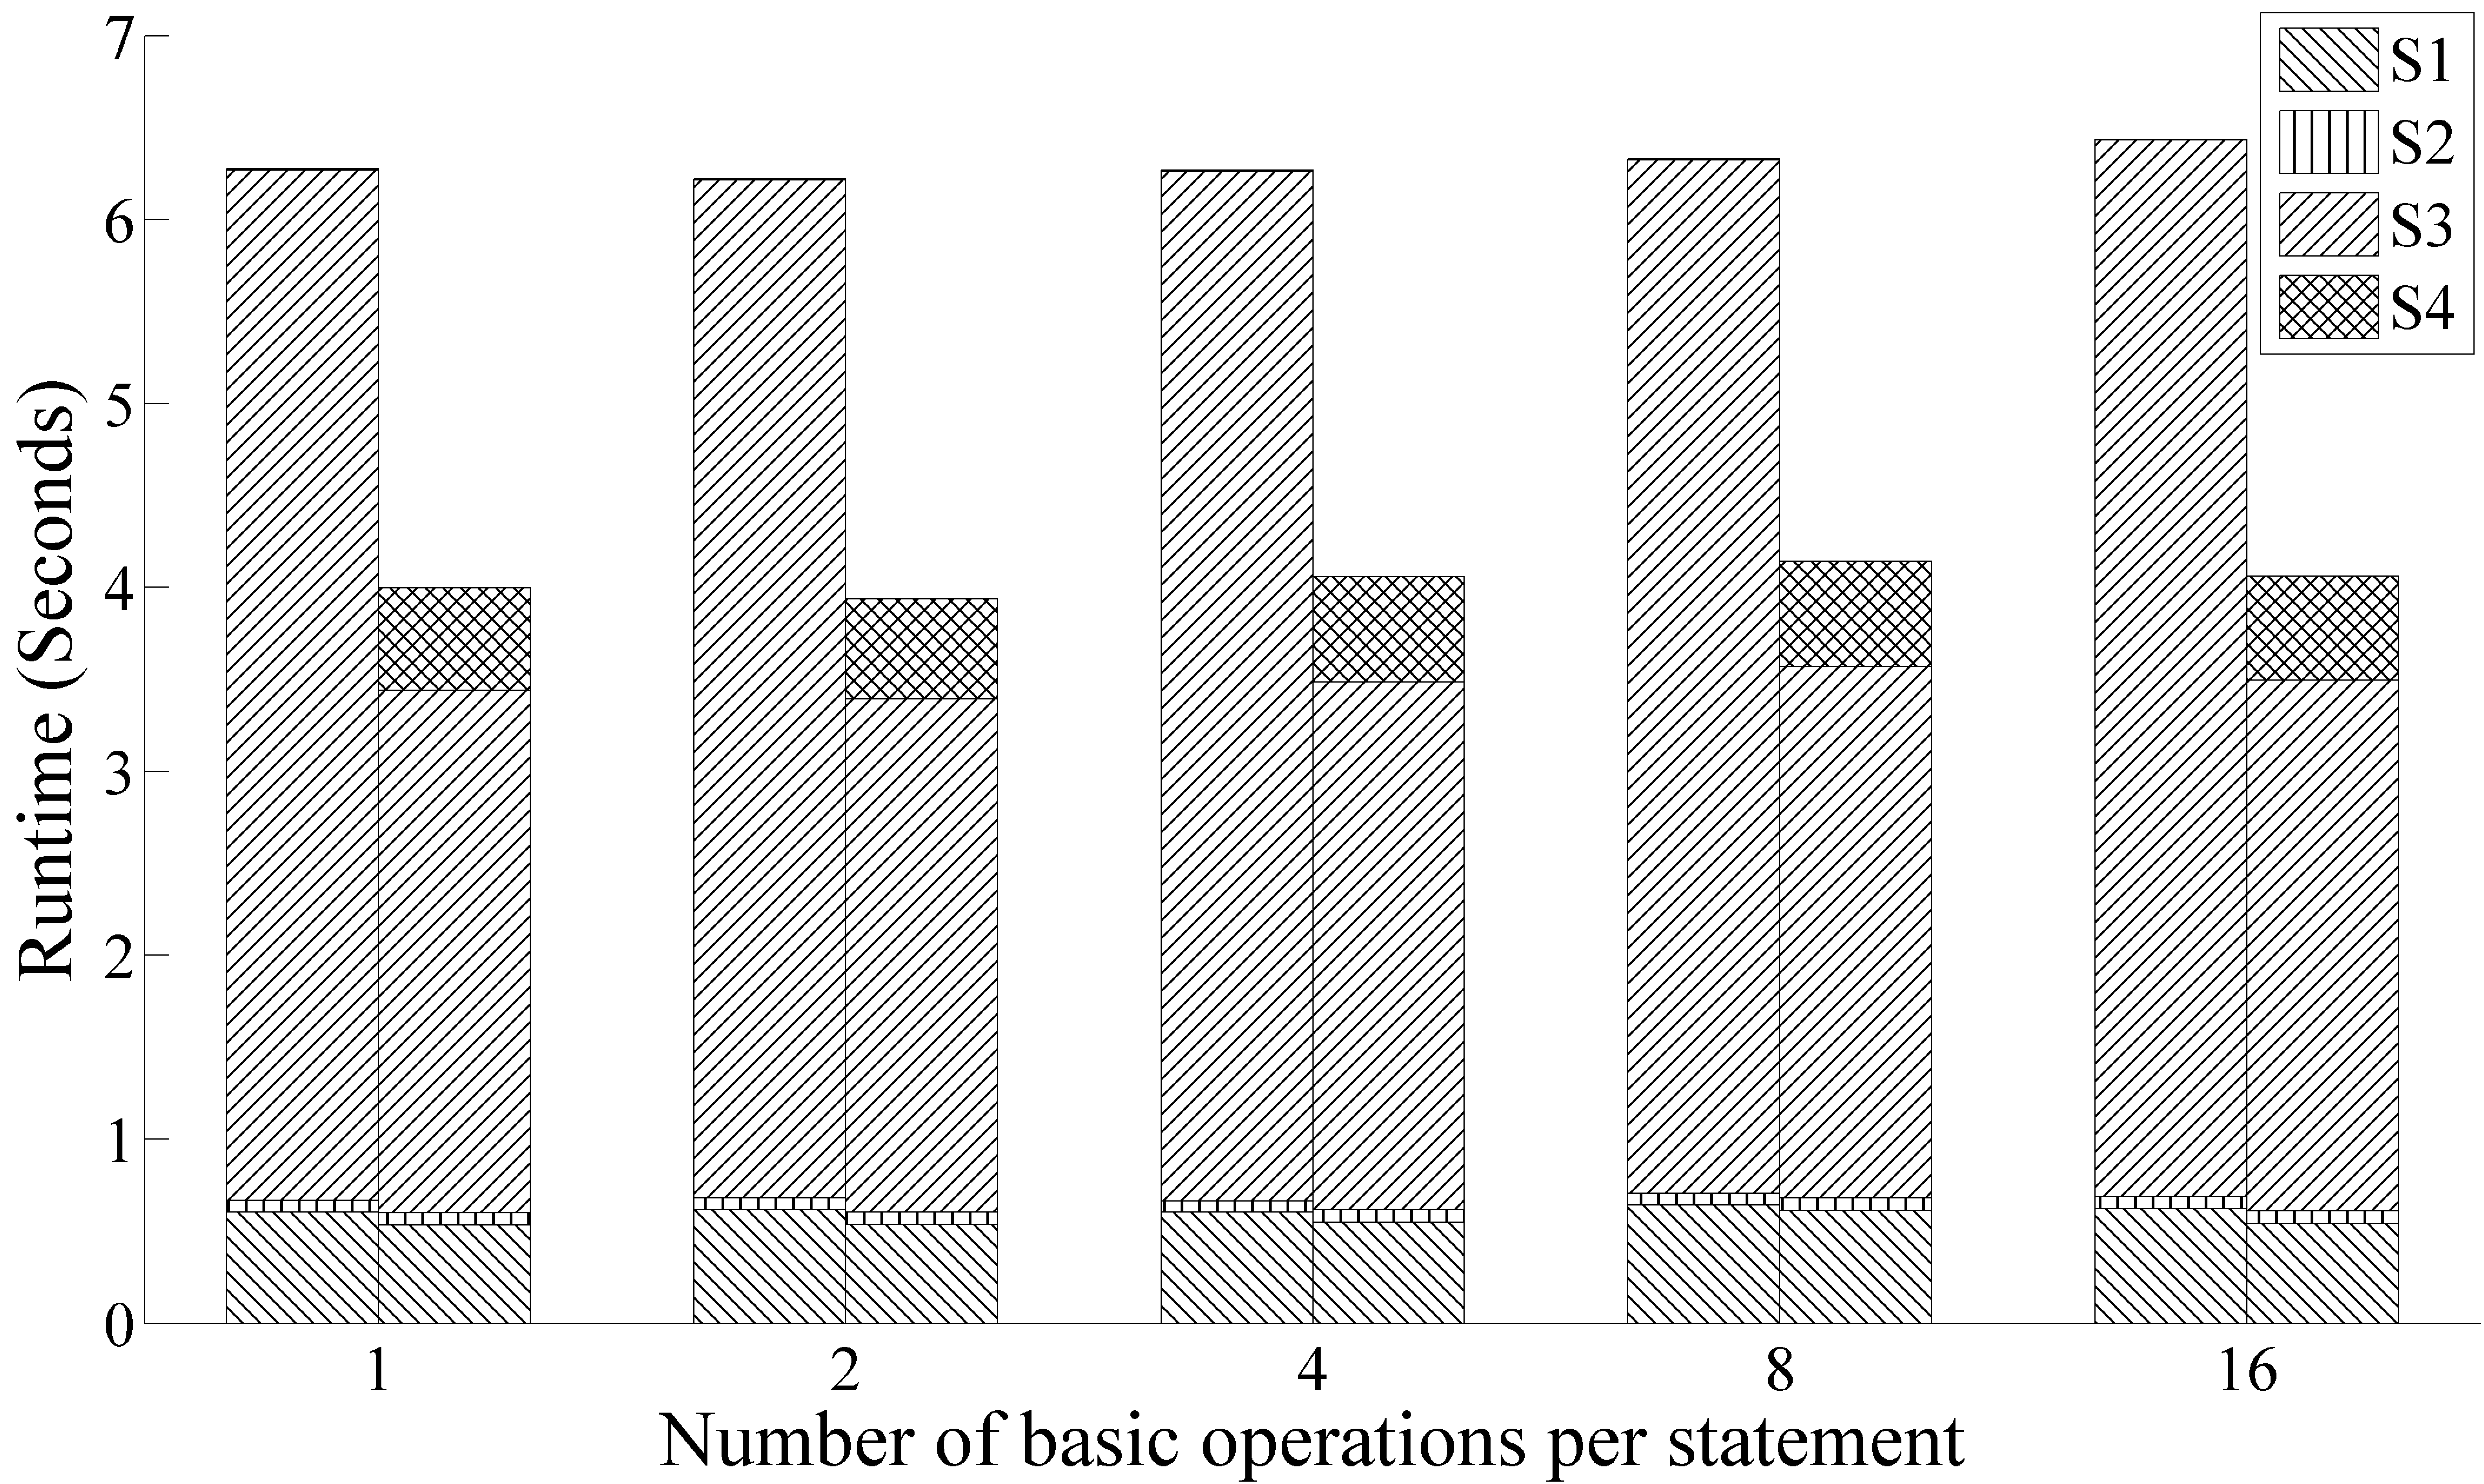
\includegraphics[width=1\textwidth]{figures/HRfig2BW}
\caption[Performance Breakdown for {\tt Direct} and {\tt Indirect} under Varying Number of Basic Operations per Loop]
{Performance breakdown for {\tt Direct} (left bar) and {\tt Indirect} methods. 
Fixed parameters: $n=20,000$, $\overline{\rho} = 6$, $B=16$. }
\label{fig:random-fig2}
\end{minipage}
\end{figure}


Figure~\ref{fig:random-fig1} shows runtime plots for the algorithms {\textsc{Livarh} and \textsc{Livarhacc} as well as
{\tt Direct} and {\tt Indirect} under this setting. We can see that {\tt Direct}, {\tt Indirect} and \textsc{Livarh} are insensitive to how the function is implemented, whereas \textsc{Livarhacc} is sensitive. In particular, the runtime of \textsc{Livarhacc} first goes down as the number of basic operations per statement increases, and then goes up. This happens because as we put 
more and more operations in a statement, we are creating more local updates and reducing the global updates.
Meanwhile the cost of each local update also increases.
As a result, \textsc{Livarhacc} performs the best when the number of operations per statement $k$ has some intermediate value, in this case, around $8$.
Beyond $k=8$, the runtime keeps increasing, and when $k=128$, \textsc{Livarhacc} surpasses \textsc{Livarh} in total runtime.


As already noted, changing $k$ does not affect the total runtime for the methods
{\tt Direct} and {\tt Indirect}. It would be interesting to see if it affects the runtime of 
any of the four constituent steps in these methods. 
In Figure~\ref{fig:random-fig2} we show the runtime breakdown for the four steps in these methods. The depicted results are for the same setting as in the previous test except that, in order to simplify the problem, we fix the total number of basic operations per loop ($B$) as $16$. We can see that changing $k$, the number of operators per statement, does not affect the runtime of any of the four steps in {\tt Direct} and {\tt Indirect}. These results are in accordance with expectation. For {\tt Direct}, the complexity of the coloring step $S2$ and the recovery step $S4$ depend only on the size and structure of the final Hessian matrix, and in general, these steps are negligible in terms of runtime compared to the steps $S1$ and $S3$. The compressed Hessian computation step $S3$ dominates the overall runtime. For {\tt Indirect}, $S2$ and $S4$ each take more time than their corresponding steps in {\tt Direct}. The step $S3$ in {\tt Indirect} takes much less time than the counterpart in {\tt Direct}, causing {\tt Indirect} to be faster than {\tt Direct}. The reason is because the time needed in $S3$ is proportional to the number of colors needed,
which in this particular case is $13$ for star coloring ({\tt Direct}) and 
$7$ for acyclic coloring ({\tt Indirect}). 

\paragraph{C) Scalability with respect to function complexity.}

We also studied the performance of these methods as we increase the complexity of the function. Since we have seen that \textsc{Livarhacc} performs the best when $k=8$, we fix $k$ to be $8$, and vary the number of statements per loop---in particular, we double the number each time. 
We use the runtime when there is only one statement per loop as a normalizing factor. 
Figure~\ref{fig:random-fig3} shows the results. 
\begin{figure}[htbp]
        \centering
        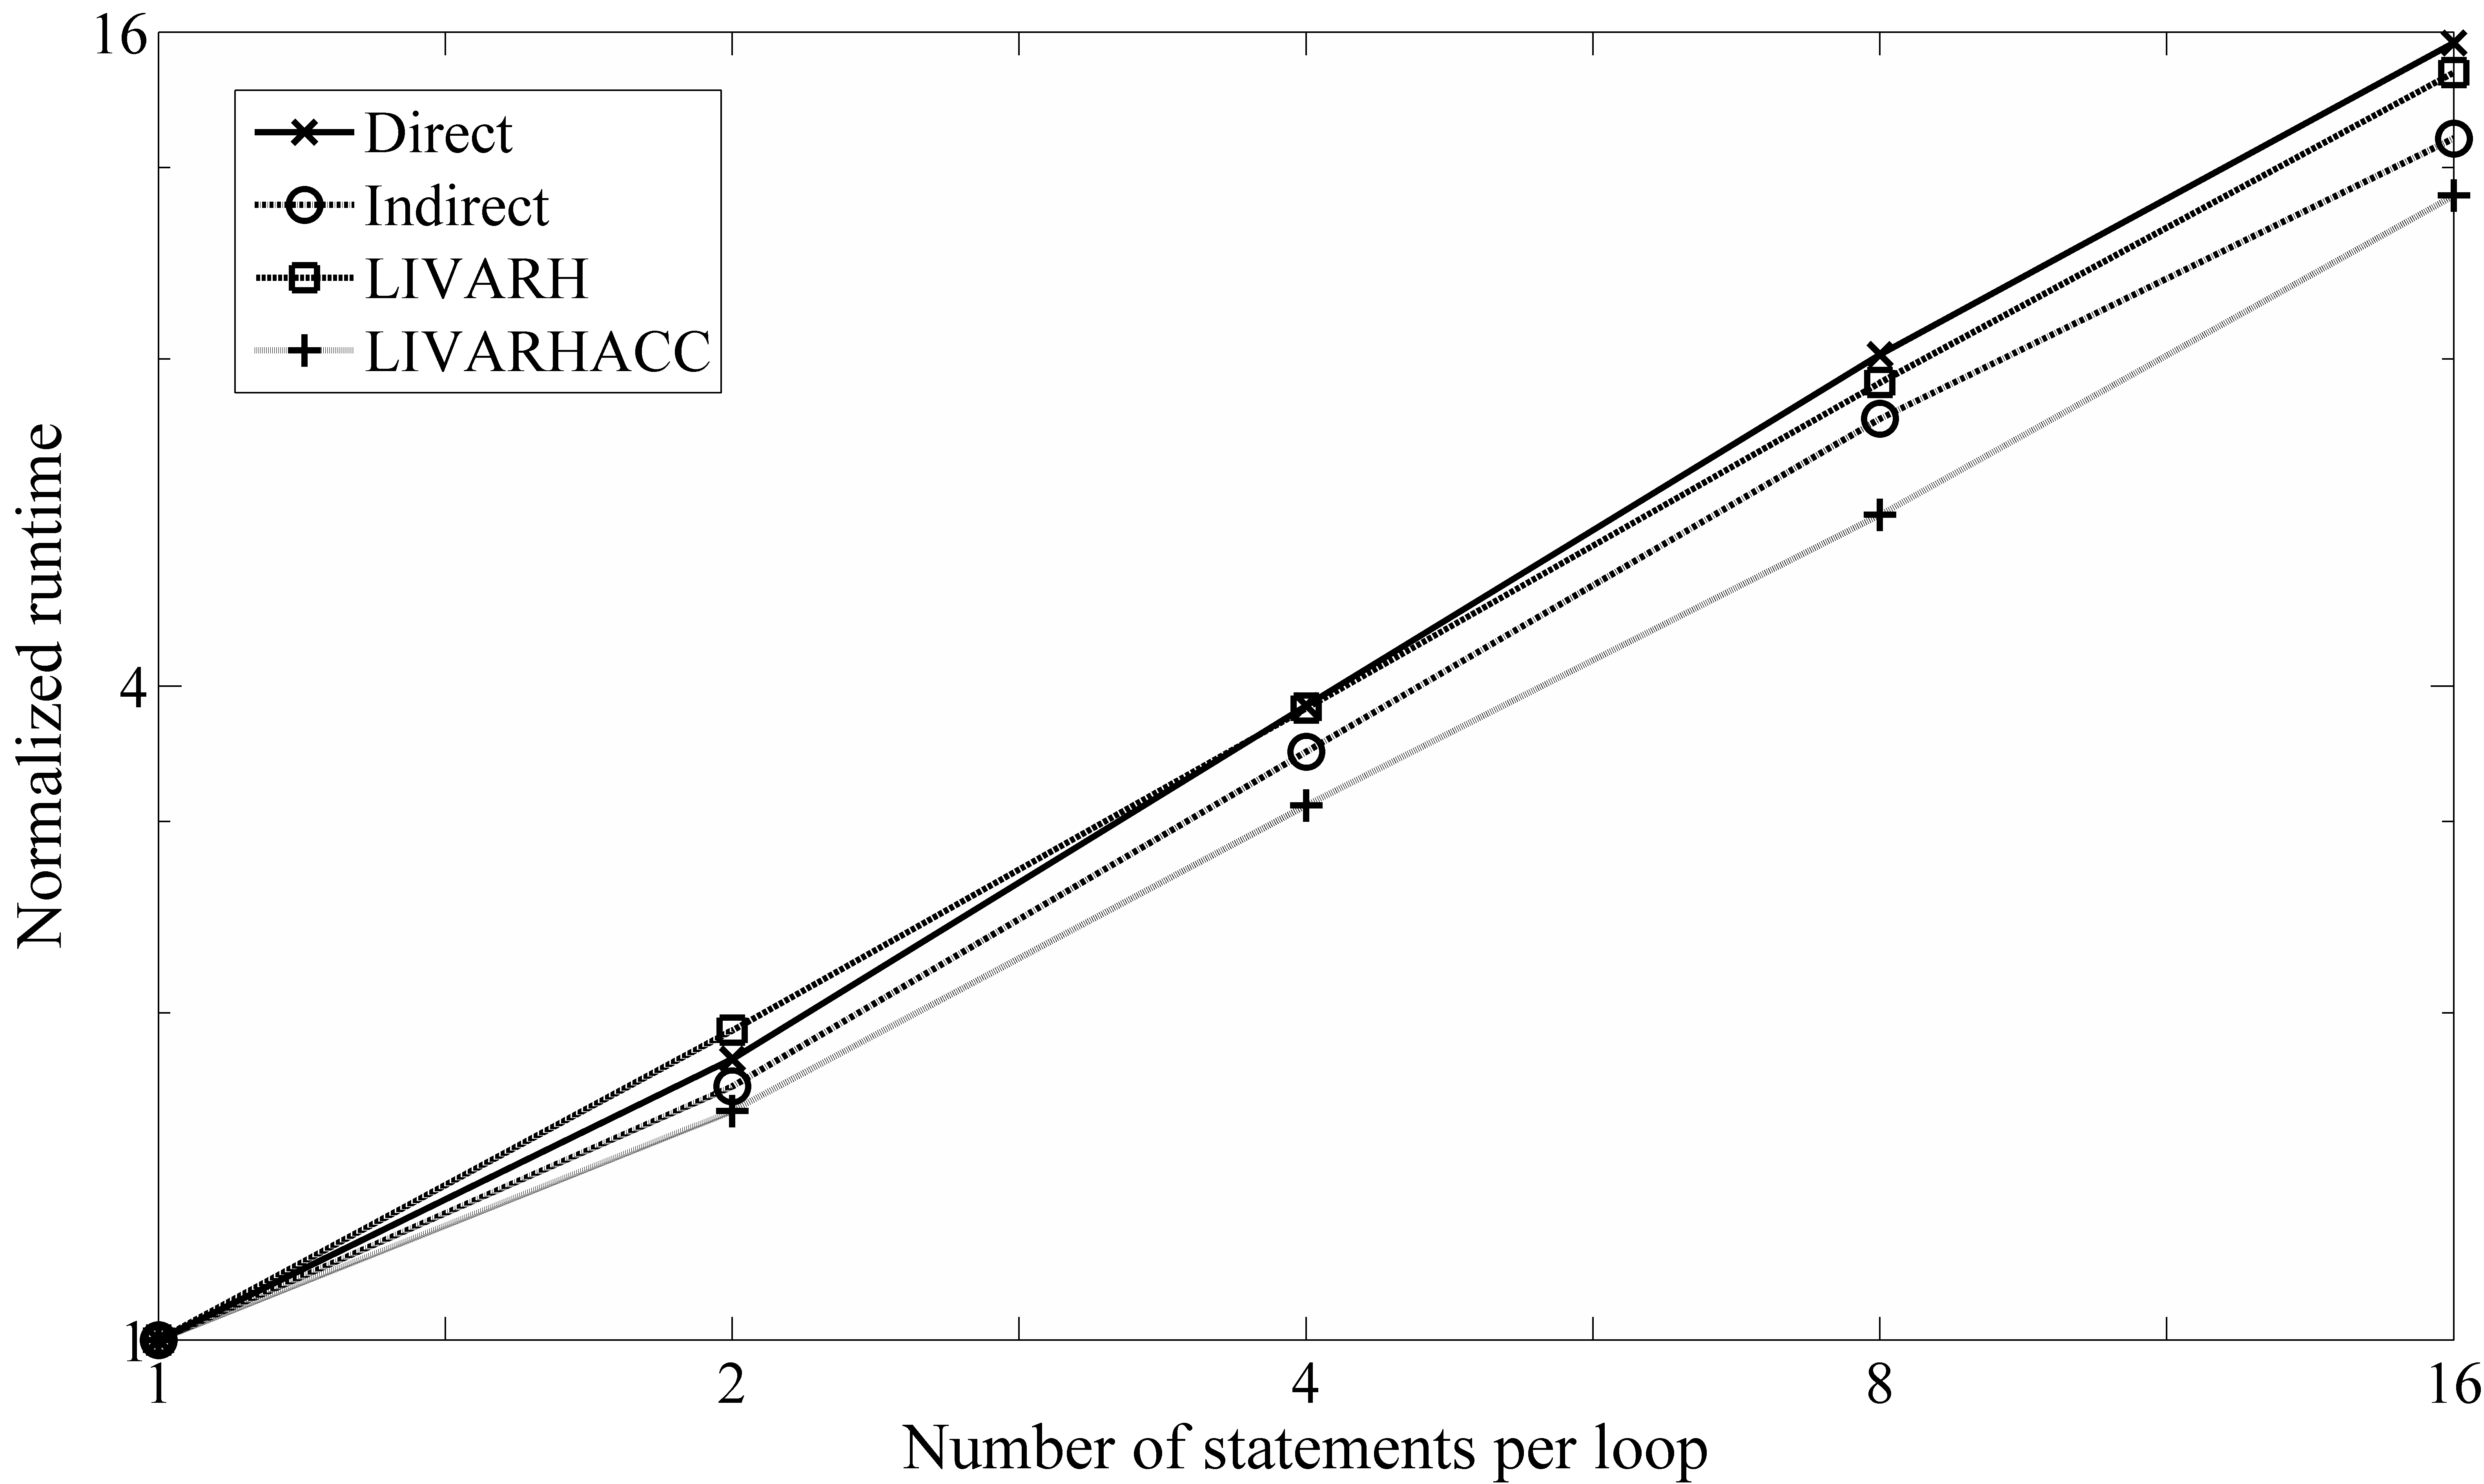
\includegraphics[width=0.65\textwidth]{figures/HRfig3BW}
        \caption[Scalability of the Different Algorithms Relative to Function Complexity]
                     {Scalability of the different algorithms relative to function complexity.}
        \label{fig:random-fig3}
\end{figure}

We observe, first, that all of these methods show linear scalability. More specifically, none of the methods needed more than twice the runtime when the complexity of the function evaluation is doubled. Further, we see that {\tt Indirect} and \textsc{Livarhacc} exhibit slightly super-linear scalability, that is, they require less than twice the runtime when doubling the complexity of the function evaluation. For {\tt Indirect}, this is because the runtime of neither the coloring step $S2$ nor the recovery step $S4$  changes when the number of statements per loop is doubled. For \textsc{Livarhacc}, the reason is when the number of identical statements in a loop increases, locality of memory accesses also increases. 


\paragraph{D) Dependence on sparsity of the final Hessian.}

In our last test, we tested how the sparsity of the final Hessian affects performance. Here, we vary the number of rows in the Hessian and approximately fix the total number of nonzeros by assigning different number of nonzeros per row in each case. We also fix the number of basic operators per loop as $8$ and the number of statements per loop as $2$. Table~\ref{tab:random-sparse} gives the structural properties of the resulting Hessian matrices.

\begin{table}[htbp]
\begin{center}
\caption[Structural Properties of Random Hessians with Varying Density but Constant $nnz$ ]
{Structural properties of random Hessians with varying density but fixed number of nonzeros.}
\label{tab:random-sparse}
\begin{tabular}{ | c | c | c | c | c | c |}
\hline
$n$ & avg & $\max$ &  $\min$ & No. colors & No. colors \\
&  $\lceil nnz/row \rceil$ &  $\lceil nnz/row \rceil$ &  $\lceil nnz/row \rceil$ & (star) & (acyclic) \\
\hline
10,000 & 12 & 25 & 6 & 26 & 11 \\
15,000 & 8 & 17 & 4 & 17 & 8 \\
20,000 & 6 & 15 & 3 & 13 & 7 \\
30,000 & 4 & 12 & 2 & 11 & 5 \\
\hline
\end{tabular}
\end{center}
\end{table}



\begin{figure}[htbp]
\centering
\begin{minipage}[b]{0.48\linewidth}
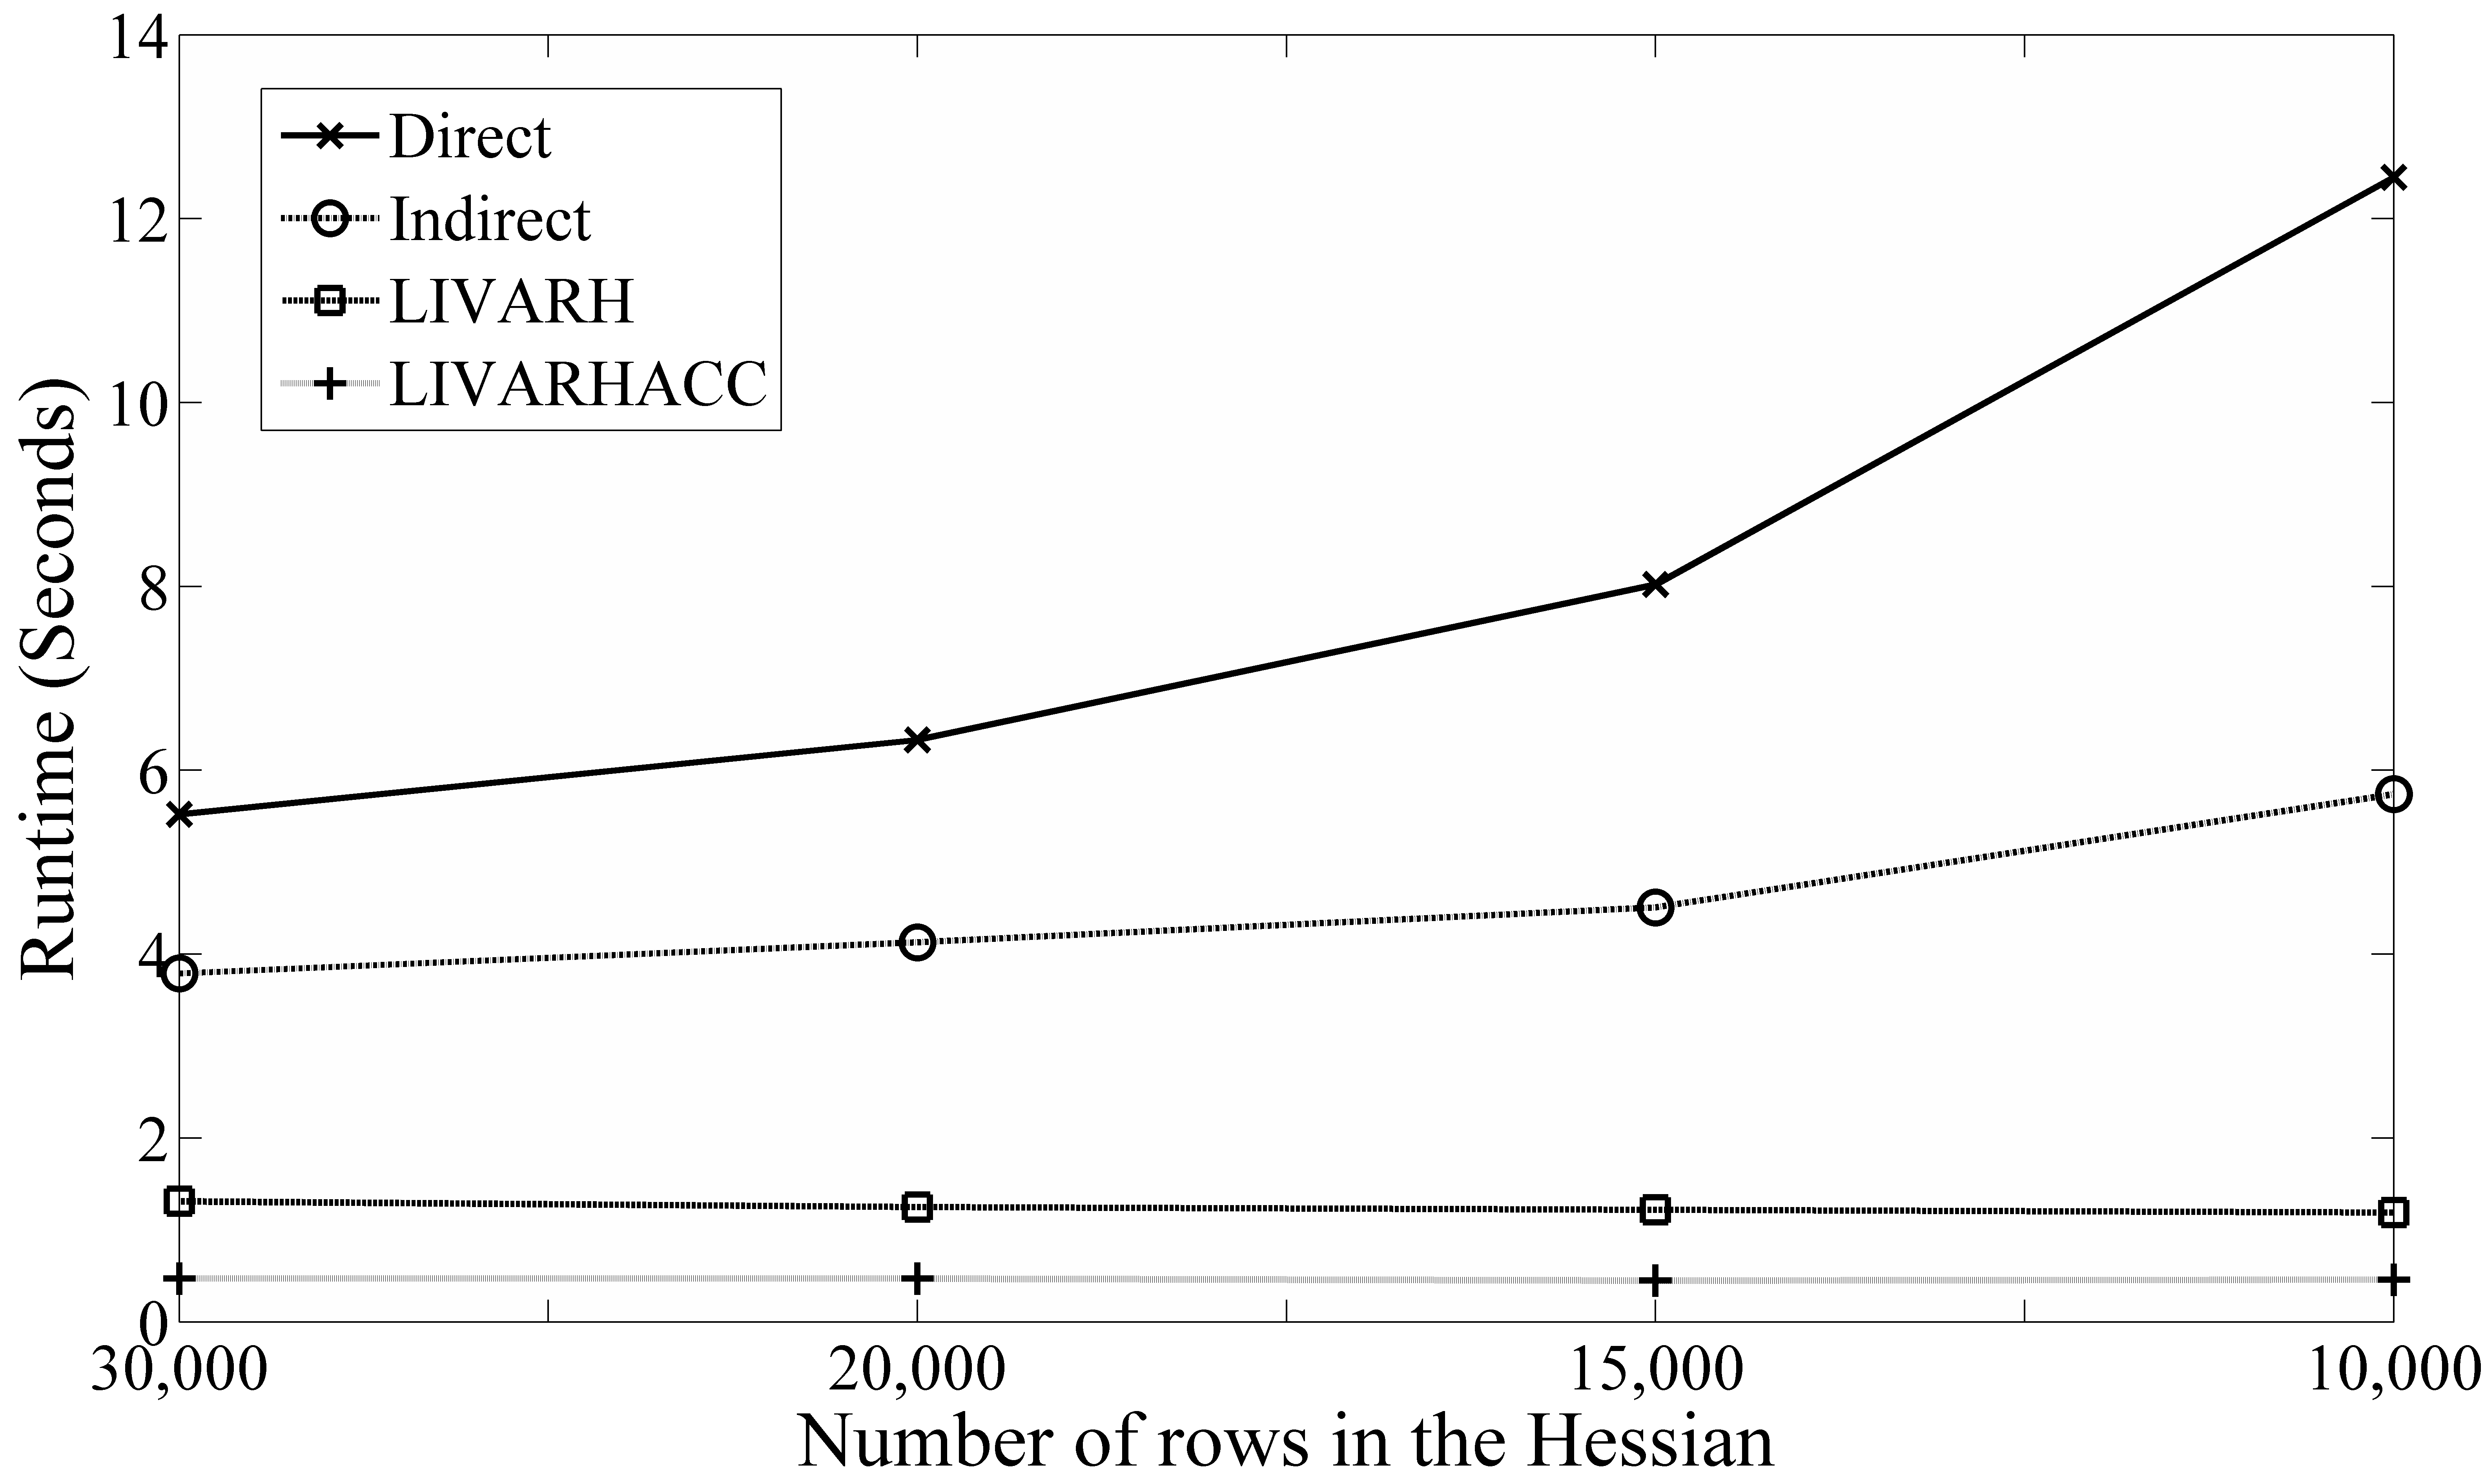
\includegraphics[width=1\textwidth]{figures/HRfig4BW}
\caption[Runtime Variation Under Different Density of Hessians]
{Runtime variation under different density of Hessians (fixed total number of nonzeros). See Table~\ref{tab:random-sparse} for structural data.}
\label{fig:random-fig4}
\end{minipage}
\quad
\begin{minipage}[b]{0.48\linewidth}
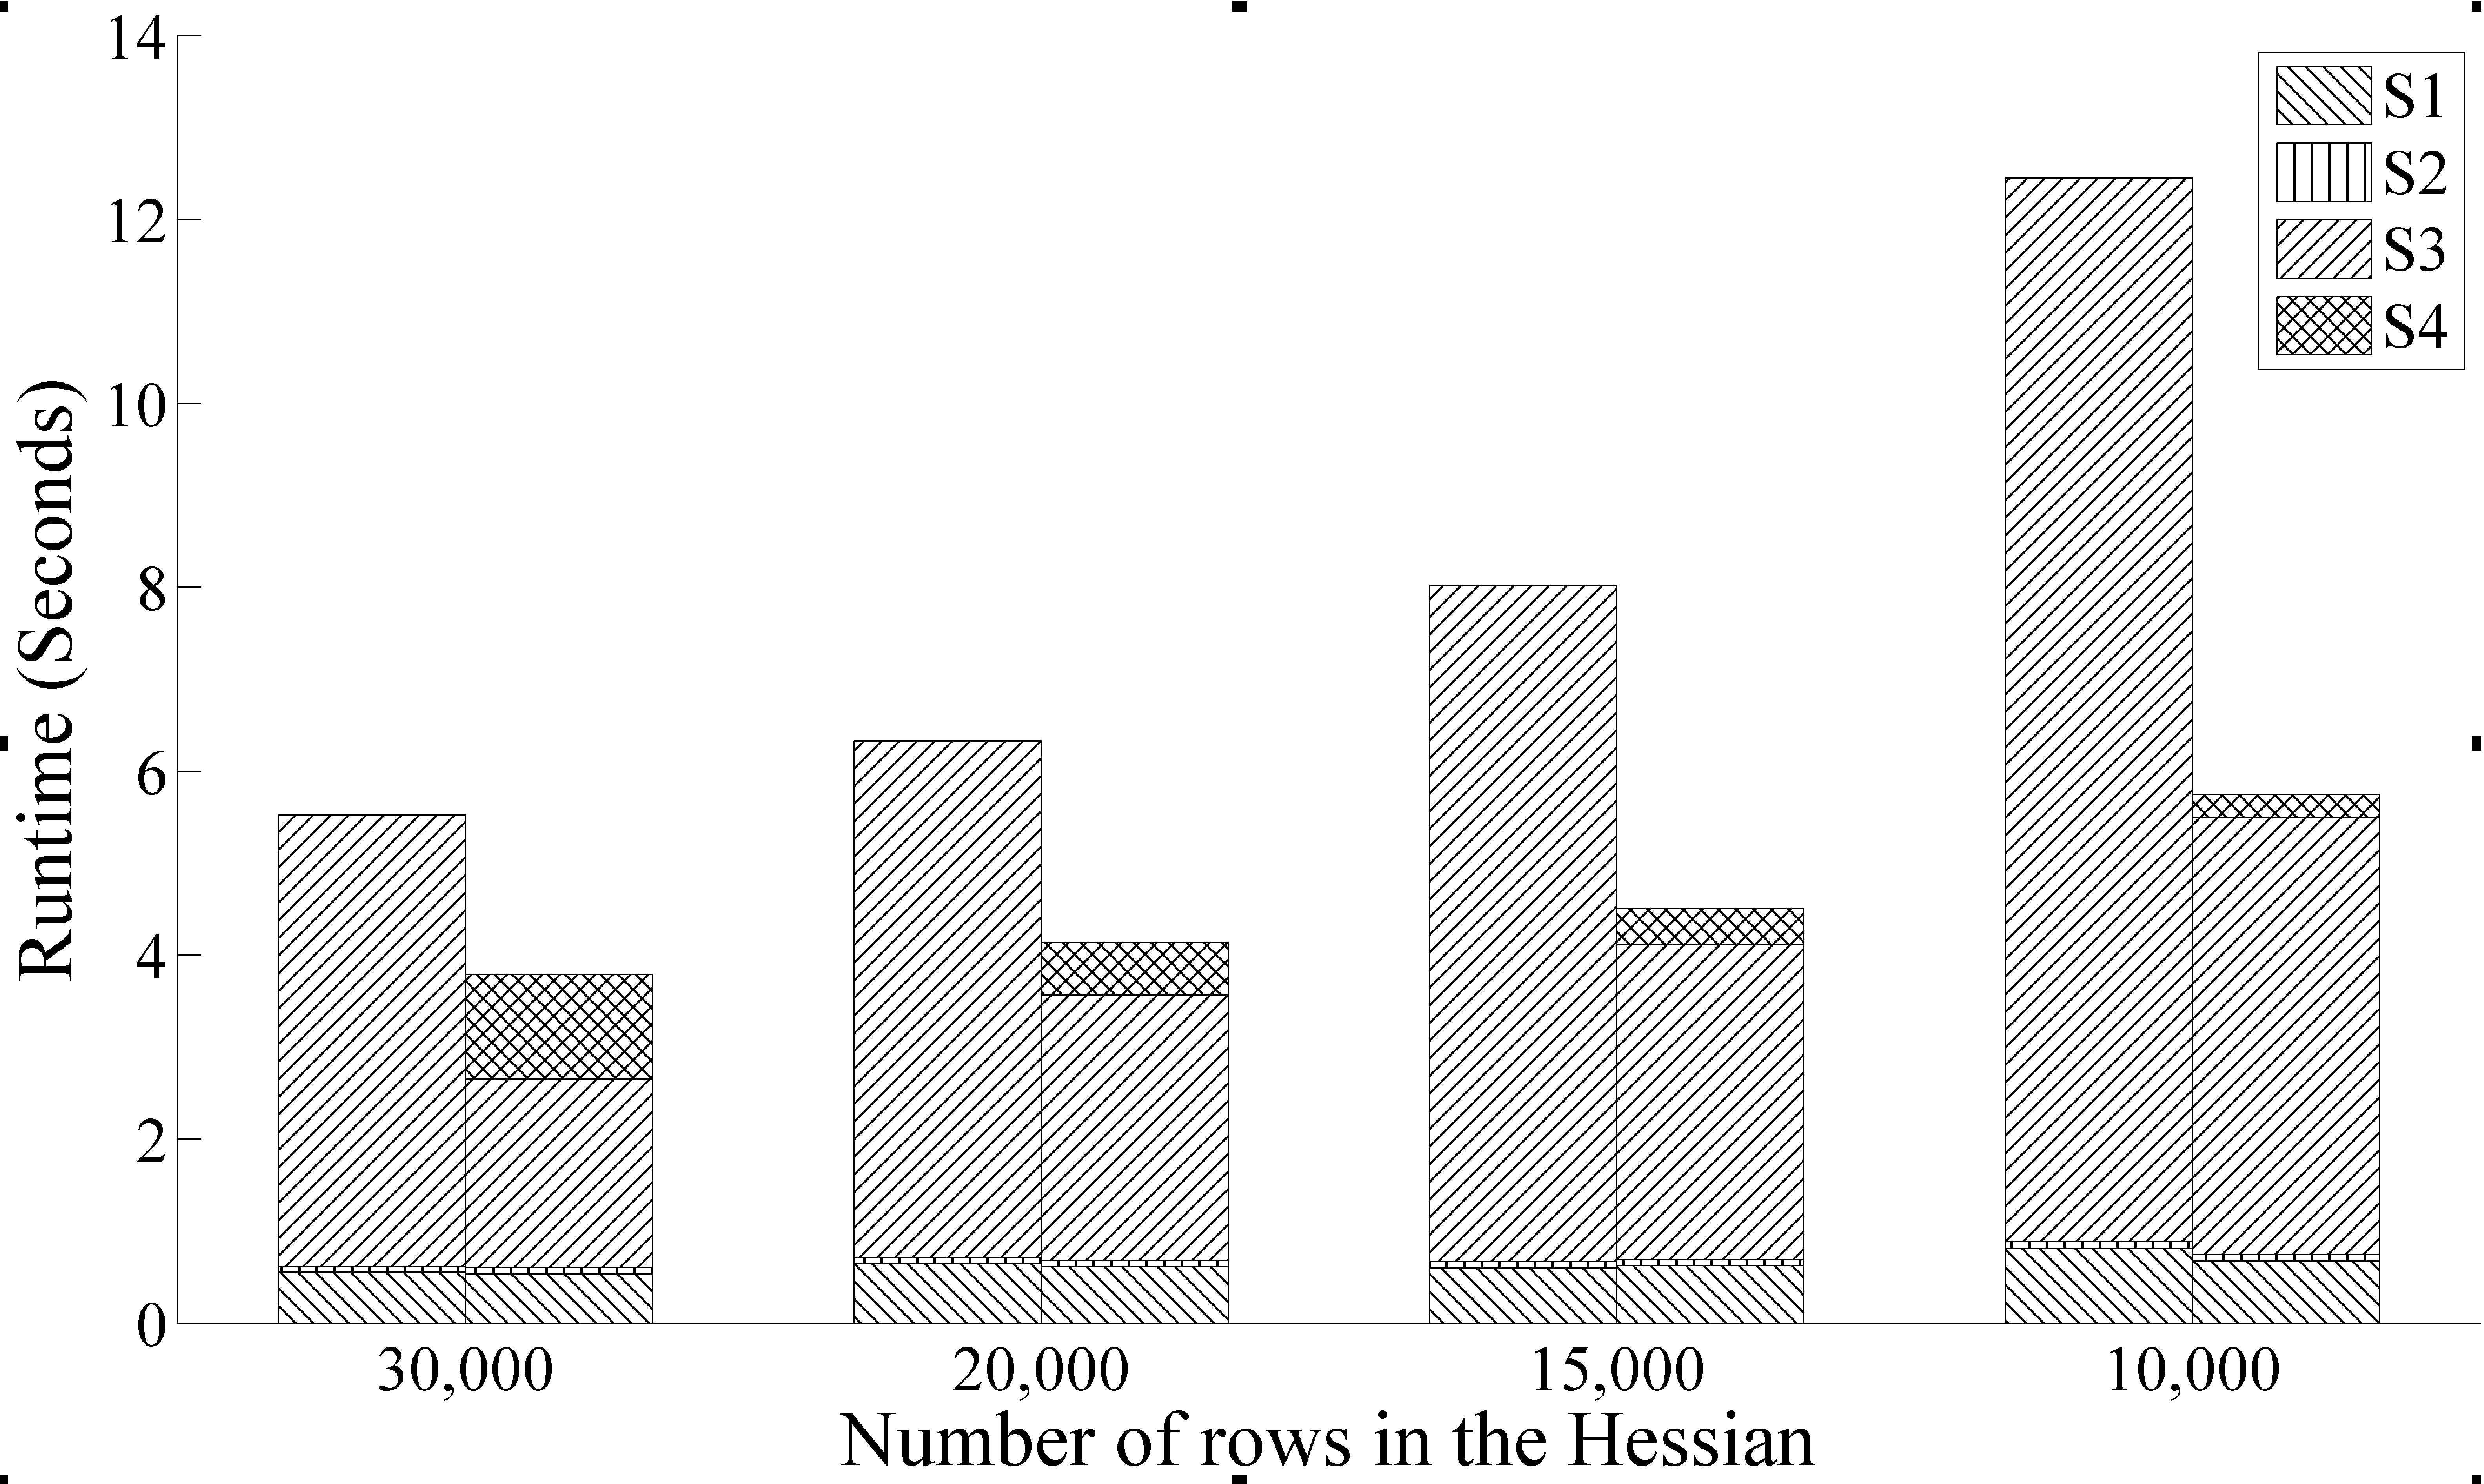
\includegraphics[width=1\textwidth]{figures/HRfig5BW}
\caption[Performance Breakdown for {\tt Direct} and {\tt Indirect} under 
Varying Density of Hessians]
{Performance breakdown for {\tt Direct} (left bar) and {\tt Indirect} (right bar) methods. Same data as in Figure~\ref{fig:random-fig4}.}
\label{fig:random-fig5}
\end{minipage}
\end{figure}

Figure~\ref{fig:random-fig4} shows runtimes for \textsc{Livarh}, \textsc{Livarhacc},
{\tt Direct} and {\tt Indirect} under this setting. 
It can be seen that the performances of \textsc{Livarh} and \textsc{Livarhacc} 
are unaffected by the changes in density. This is as expected because the complexity of these
algorithms is only determined by the number of SACs. The runtime of {\tt Direct} and {\tt Indirect} increases as the density of the Hessian matrix increases. Figure~\ref{fig:random-fig5} shows the runtime breakdown for {\tt Direct} and {\tt Indirect}. For {\tt Direct} the runtime 
is dominated by step $S3$, which in turn is proportional to the number of colors needed. As the Hessian size is decreased while keeping the total number of nonzeros fixed, the matrix gets denser and so we need more colors. As a result, {\tt Direct} would need more time to evaluate the compressed Hessian. For {\tt Indirect}, the runtime for the recovery step $S4$ decreases when we have a Hessian matrix of smaller size, but the increase in the time for step $S3$ still dominates the overall runtime.

\subsection{Pseudocode of The Random Hessian Generator}
\label{sec-random-code}

The pseudocode of the random Hessian generator is given in Figure~\ref{fig:RandomHessianGenerator}.

\begin{figure}
\begin{center}
\begin{tabular*}{\textwidth}{l}
\hline
\textbf{Algorithm:} Random Hessian Generator \\  
\hline
\begin{minipage}{3in}
\begin{verbatim}
// x : array of independent variables
// y : dependent variable
// n : size of the Hessian, y''
// p : half of the average number of nonzeros per row

#define EXP_1 (1.0+x[i]*x[j])  // 1 basic operation to create a nonzero entry
#define EXP_2 EXP_1+EXP_1  // sum of 2 basic operations
#define EXP_4 EXP_2+EXP_2  // sum of 4 basic operations

#define STMT_1_4 y+=EXP_4;  // 1 statement containing 4 basic operations
#define STMT_2_4 STMT_1_4;STMT_1_4;
#define STMT_4_4 STMT_2_4;STMT_2_4;
#define STMT_8_4 STMT_4_4;STMT_4_4;

adouble function random_hess_generator(adouble* x, int n, int p) {
  adouble y=0;
  for(i = 0; i < n; i++) {
    for(l = 0; l < p; l++) {
      j = randomIndex();
      STMT_8_4;  // 8 statements, each containing 4 basic operations
    }
  }
  return y;
}
\end{verbatim}
\end{minipage} \\
\hline
\end{tabular*}
\end{center}
\caption[The Random Hessian Generator]{The Random Hessian Generator. Note that the equivalent mathematical expression is: $y=f(x)=\sum_{i=1}^{i=n} \sum_{l=1}^{l=p} 32 (1.0 + x[i] \times x[j_{il}])$, each $j_{il}$ is randomly chosen from the interval $[1, n]$.}
\label{fig:RandomHessianGenerator}
\end{figure}

\end{document}